\documentclass[10pt,final,journal,a4paper,oneside,twocolumn]{IEEEtran}
\usepackage{hyperref}
\usepackage[numbers]{natbib}
\bibliographystyle{IEEEtran}
\usepackage{amsmath,amssymb,amsfonts}
\usepackage{algorithmic}
\usepackage{graphicx}
\usepackage{textcomp}
\usepackage{xcolor}
\usepackage{tabularx}
\usepackage{booktabs}
\usepackage{comment}
\usepackage{minted}
\usepackage{xurl}
\usepackage{adjustbox}

\providecommand*{\listingautorefname}{Listing}
\def\BibTeX{{\rm B\kern-.05em{\sc i\kern-.025em b}\kern-.08em
    T\kern-.1667em\lower.7ex\hbox{E}\kern-.125emX}}

\begin{document}

\title{Exploring Deep-Learning Recommender Systems for Book Recommendations}

\author{\IEEEauthorblockN{1\textsuperscript{st} Simon Müller}
\IEEEauthorblockA{\textit{M.Sc. Computer Science student, Data Science class} \\
\textit{University of Applied Sciences Augsburg}\\
Augsburg, Germany \\
simon.mueller3@hs-augsburg.de}}

\maketitle

\begin{abstract}
In this paper, a deep-learning-based recommendation system for recommending books is presented. A Deep \& Cross Network architecture is used to predict a user's book rating which can then be used to rank recommended books. Extensive textual features about the items are included using word embeddings to increase the information available from which to infer the recommendations. Hyperparameter optimization is then carried out to find the best configuration for the model.
\end{abstract}

\begin{IEEEkeywords}
deep learning, recommendation, neural networks, recommender systems, deep \& cross network, hyperparameter tuning
\end{IEEEkeywords}

\section{Introduction}
The current time has been described not only as the "information age", but also as an attention economy. Corporations compete for the limited attention of their prospective customers. On social media platforms, users have to be made to spend as much time as possible on the services so as much data on them as possible can be gathered and more advertisements can be shown. Subscription services want to present their users with perfectly fitting content to keep them interested in their platform and subscribed to their service. Online warehouses have an even more direct interest in providing the best fitting products to customers to directly influence their sales.

Recommendation systems are used especially in the advertising and sales business domains. There, they are used to predict click-through rates on ads, which is the probability of a user interacting with a displayed online advertisement. This is of utmost importance for advertisement providers like Alphabet or Meta, which can increase their advertisement prices based on how well they know their potential advertisement target audience. 

For all of these examples, the users of the respective platforms and services have to be recommended the most appropriate products, pieces of content, or advertisements to keep the user's interest in the service. This task is the goal of the recommender or recommendation systems, which will be explored in this paper on a concrete data set.

\section{state of the art}\label{sec:stateoftheart}
As described in the Introduction, most interest in the topic arises in the advertisement and sales business, which is why a lot of research is being done by the research departments of Google, Meta (formerly Facebook), Microsoft, and Amazon.

In the following section, a general ontology of recommendation systems will be presented.
There are two main types of classic recommendation methods, Content-based Filtering and Collaborative Filtering. They differ in their main goals and the data available. 
Collaborative Filtering on one hand tries not to perfectly know the specific item the targeted user may be most interested in but instead tries to best categorize the user base into different groups with similar interests. This is done because users with similar general interests generally respond the same to specific recommended items, and often a "perfect fit" is unnecessary or virtually impossible to achieve because of the sparsity of the available data.
Collaborative Filtering methods are especially useful for predicting click-through rates for advertisements, because in this context, usually, only implicit feedback is available. Implicit feedback is feedback data tracked by cookies with only relatively insignificant correlations. A click on a search result or an item on a shopping website, or a like on a social media post are considered implicit feedback.  When the data consists of millions of these small interactions, this implicit feedback may be used to give explicit recommendations. For this approach, a huge data set is needed, since a single click is of little value, because i.e. it may be a misclick without any relevance to the user. Implicit feedback dataset matrices usually consist of thousands of features, which are occupied only very sparsely.


Content-based filtering on the other hand instead tries to achieve the opposite. These algorithms take as much information available about the items (the content) as possible to predict the interest of a user for it, or the likelihood of an interaction respectively. These approaches usually rely on explicit feedback by the users, which makes predictions more predictable. They are used in domains like streaming services, where for example the service provider can estimate if the user liked a movie if he watched it completely, and especially if the user gives an explicit item rating, usually on a 1-5 stars or at least a like/dislike basis.

A basic approach to predict these likelihoods is to estimate a user-item matrix, with each unique user as a row and all the available items as columns, where the matrix cells [i,j] are filled with a calculated probability of interaction or the predicated rating or similar interest indicator. 

Deep-Learning-based systems try to combine these approaches while letting a deep neural network architecture take care of the feature selection to gain the best recommendations.

\section{related work}
The survey \cite{Zhang.2020} provides a very in-depth review of current deep-learning-based recommender system approaches using all kinds of deep learning algorithms and network structures from CNNs, GRUs, Deep Factorization Machines, to Reinforcement-Learning- and Attention-based systems.

For this work, the Deep \& Cross Network \cite{Wang.2017} \cite{Wang.2021} developed by researchers at Google was used. This network was mainly chosen because of an existing tutorial and basic sample implementation in the Tensorflow framework.
Initially, a comparison between different recommendation architectures like Neural Collaborative Filtering \cite{He.2017}, developed at the University of Singapore, Wide \& Deep learning \cite{Cheng.2016} by Google and DLRM \cite{Naumov.31.05.2019} by Facebook researchers, was planned.
Unfortunately finding running implementations in the current Tensorflow version 2, using similar programming interfaces (since Tensorflow provides a few different ways to provide data and define models), and adapting them to the available dataset proved to be way more complicated than anticipated, which is why the idea had to be abandoned in the end.


\section{research question}
The goal of this work was to develop a recommendation system to recommend books to users, based on the \emph{"UCSD~Book~Graph"} data set, which will be further introduced in \autoref{sec:data}. The main challenges were to decide which data to use, how to prepare it and feed it into the artificial neural network, and to find out which hyperparameter configuration and data features result in the best recommendation performance.
An important part of this task was the inclusion of textual features of different lengths and complexity, which had to be preprocessed and embedded.


\section{model architecture}\label{sec:model_arch}

\begin{figure}[ht]
    \centering
    \includegraphics[width=\linewidth]{dcn_architecture}
    \caption{Visualization of two kinds of DCN-V2-architectures. $ \bigotimes $ represents the cross operation~\cite{Wang.2021}.}
    \label{fig:dcn_arch}
\end{figure}

\autoref{fig:dcn_arch} shows two variants of the Deep \& Cross Network architecture as defined in \cite{Wang.2021}. For this paper, the "Stacked" approach was used.
In both of them, the network consists of three parts. 
First, in the Embedding Layer, for sparse (categorical) features, dense embeddings are learned and then concatenated to dense (numerical) features to create the network input. These features are then fed into the cross sub-network, in which feature interactions using the cross layers are modeled. After passing through an activation layer, these crossed features are passed to the second, deep sub-network, in which deep densely connected layers are used. After a final activation function appropriate to the problem on hand (softmax for multi-class classification, linear for regression), the final output can be received from the model.

The cross-network applies feature crossing at each layer, with cross orders (polynomial degrees) increasing with layer depth. \autoref{fig:dcn_cross} shows the $ (i+1) $-th cross-layer.
$ x_{0} $ is the base layer (embedding layer), $ x_{i} $  is the input to the cross layer, $ \bigodot $ represents element-wise multiplications, and matrix $ W $ and vector $ b $ are the parameters to be learned.

\begin{figure}[ht]
    \centering
    \includegraphics[width=\linewidth]{dcn_cross}
    \caption{Cross layer visualization~\cite{Wang.2021}.}
    \label{fig:dcn_cross}
\end{figure}

For a more detailed description of the model and the used cross layers, one may refer to the original papers or the simpler explanation in a TensorFlow Blog post~\cite{Wang.2020}.


\section{technology stack}
The implementation and initial training of the deep learning-based recommender system presented in this work was carried out on a local machine running Windows 11 and was later moved to a more performant Unix-based machine hosted by the University of Applied Sciences Augsburg, its "daenerys" server.
The programming was done in python, the most commonly used programming language in this field, using Jupyter Notebooks for easier interactive experimentation. For data preprocessing and cleaning, the \emph{pandas} library was used.
\emph{Tensorflow} was used as the machine learning framework to implement both the data processing pipeline as well as the deep learning recommendation system models. For the data input and processing pipeline, the \mintinline{python}{tf.data} TensorFlow interface was used.


\section{data set}\label{sec:data}
The data set used for this work is the \emph{"UCSD~Book~Graph"}~\cite{Wan.2018}~\cite{Wan.2019}, created at the University of California, San Diego (UCSD).
The dataset was scraped in late 2017 from the website goodreads.com and last updated in 2019 and consists only of publicly available data. Goodreads is a social media platform where users can create virtual bookshelves to show their book collections, track their reading progress, discuss books in forums and create text reviews for the books they've read. Goodreads was launched in 2006 and has since been bought by Amazon in 2013. The platform has over 90 million users as of 2019.

The provided dataset is of enormous size, containing information about more than two million books, more than 800k users, with more than 200 million interactions between the latter.
Because of the sheer scale of the data set, the authors recommend using only a subset of the data, especially when used on a local machine. For this, they have created subsets for different genres, like \emph{"Children"}, \emph{"History \& Biography"} or \emph{"Mystery, Thriller \& Crime"}. These categorizations may not be perfect and may overlap, since a genre specification is not directly available in the book metadata, but is instead inferred from the shelves users have put the books on.
From this gigantic dataset, only a subset was read in the preprocessing process, as will be described in \autoref{sec:data_preprocessing}.

\subsection{Books}
The book data set contains 2.36 million entries, including information like a unique ID, title, author, release date, and a description text. A sample of all the available columns is shown in \autoref{tab:book_sample} in the Appendix. As shown in the table, not every column is available for all data points.
For building this recommender system, only the following columns were deemed to be useful and used consequently:
\begin{itemize}
    \item title
    \item number of text reviews (popularity)
    \item average rating
    \item description text
    \item author ID
\end{itemize}

\subsection{Shelves}
Users of the Goodreads website may categorize their books into different shelves. Some of them may be exclusive. The most prominent shelves are the three pre-defined shelves "to-read", "read", and "want-to-read". On top of that, users may add as many shelves as they like and place books into one or more of them to keep track of their book collection.
The shelf-interaction dataset may be used as implicit feedback, as described in \autoref{sec:stateoftheart}. As stated previously, the dataset is very large and sparse. A user having shelved a book does not necessarily imply strong interest in the book, but it is an indicator. 
The data consists of mappings between user ID and book ID, with additional indicators if the book has been read (inferred from the existence of the book on the "read" shelf), the user's rating if available, and if the user created a review on it. These additional indicators may be used as explicit feedback.
A more detailed data set adds time information to this, recording when the user has started and finished the book. The authors of the dataset themselves have used this data to create a recommender system using time series data \cite{Pera.2018}.

\subsection{Reviews}
On top of the book metadata and basic user interactions with these books, textual reviews have been scraped. The complete dataset contains multilingual review text without spoiler tags. It contains more than 15M reviews about ~2M books and 465K users. Users of the website can add spoiler tags to hide sensitive plot information from other readers, these tags have been removed from the dataset. This data was used to train a neural network to autonomously detect spoilers in text data \cite{Wan.2019}.

The columns of this data are shown in the sample \autoref{tab:review_sample} in the Appendix. It should be noted, that only about 40 percent of the available 1.3 million review text data points were used to limit the performance impact and training times for training models on such large scale data.
From the review data available, only the following columns were used:
\begin{itemize}
    \item user ID
    \item book ID
    \item rating
    \item review text
\end{itemize}

\subsection{authors}
There is a separate data set available for author information, e.g. their names, number of reviews to their books, and their average rating. This information was not used, since the author's id as a unique identifier was deemed as sufficient information, whereas specific book (item) features seemed to be of greater importance.

\subsection{Data subset used in this work}\label{sec:data_used}
As described in the preceding paragraphs, the provided dataset is of an industrial scale. To explore the data and train neural networks in a reasonable time, only a subset of data is used.
The \emph{Mystery, Thriller \& Crime} subset was chosen for this work. It consists of 219,235 books and 1,849,236 detailed text reviews. The interaction data was not used, because the main point of interest in this work was to learn recommendations based on explicit content information, like the item descriptions, and not to imitate recommender systems used e.g. for ad-click-prediction using implicit interactions feedback.

\begin{table}[h]
    \centering
    \caption{combined dataset}
    \label{tab:all_data}
        \begin{tabular}{clll}
                \toprule
                Column & \# Unique Values \\
                \midrule
                user\_id & 93480  \\
                book\_id & 152258\\
                rating & 6\\
                review\_text & 956133\\
                title & 99813 \\
                text\_reviews\_count & 1715 \\
                average\_rating & 296 \\
                description & 123034 \\
                author\_id & 25548 \\
                \bottomrule
        \end{tabular}
    \end{table}

\section{Data Processing}\label{sec:data_preprocessing}
\subsection{data cleaning and preprocessing}
As part of the data cleaning process, the pandas columns were cleaned "on the fly" while converting the JSON data into CSV.
The conversion to CSV was necessary because the \mintinline{python}{pandas.read_json()} implementation does not bode well with large JSON files with a single item per line in the file. Reading JSON like this leads to the RAM getting clogged up until the process finally collapses. Reading potentially gigantic CSV files into a DataFrame all at once on the other hand poses no problem at all to the library.

First, the review id and book id respectively are used as the table indices. For the book information, only five of the available columns are used. Temporal information, like "date added", "read at", is removed from the review dataset, since taking this information would necessitate a different, sequential model architecture with some kind of recurrence.
For the remaining columns of the CSV dataset, fitting datatypes are set (instead of using the all-encompassing "object" type) and escaped characters in longer texts are replaced by empty spaces.
The two separate DataFrames are finally merged into one based on their common book IDs. Rows that contain empty column values or NaN data are dropped, which leads to the final dataset size as shown in \autoref{tab:all_data}.

Excerpts of the data preparation process are shown in \autoref{lst:data_loading} and \autoref{lst:data_prep}.

\begin{listing}[h]
    \begin{minted}[breaklines,fontsize=\footnotesize]{python}
chunk_size = 500
book_reader = pd.read_json(os.path.join(DIR, in_fn_books), lines=True, dtype={
    "title": 'string', 
    "description": 'string', 
    "text_reviews_count": 'uint', 
    'average_rating': 'float'
}, chunksize=chunk_size)

def prepare_book_df(df):
    df.set_index("book_id", inplace=True)
    df.loc[:,'author_id'] = df['authors'].apply(lambda row: row[0]['author_id']) # just select the first author_id of the list of authors
    df.loc[:, 'author_id'] = df['author_id'].astype('int64')
    df = df.loc[:, ['title', 'text_reviews_count', 'average_rating', 'description', 'author_id']]
    df.loc[:,'title'] = df['title'].str.encode('utf-8')
    df.loc[:,'description'] = df['description'].replace(r'\n',' ', regex=True) 
    return df

# write first chunk with header
with open(os.path.join(OUT_DIR, "books.csv"), 'a') as f:
    chunk = next(book_reader)
    chunk = prepare_book_df(chunk)
    chunk.to_csv(f, header=True, line_terminator='\n')  
# process the rest of the data
with open(os.path.join(OUT_DIR, "books.csv"), 'a') as f:
    no_lines = 219235
    for chunk in tqdm(book_reader, total=no_lines/chunk_size):
        chunk = prepare_book_df(chunk)
        chunk.to_csv(f, header=False, line_terminator='\n')

# (...) repeat similarly for review data
    \end{minted}
\caption{\small Data cleaning process for converting JSON to CSV}
\label{lst:data_loading}
\end{listing}
\begin{listing}[h]
    \begin{minted}[breaklines,fontsize=\footnotesize]{python}
book_dtype={
    "title": 'string', 
    "description": 'string', 
    "text_reviews_count": 'uint', 
    'average_rating': 'float'
}
review_dtype = {
'book_id': 'uint32',
'rating': 'uint8',
'review_text': 'string',
}

df_books = pd.read_csv(os.path.join(DIR, csv_fn_books), dtype=book_dtype, low_memory=True)
df_books.title = df_books.title.str.strip("b\'\"") 
df_reviews = pd.read_csv(os.path.join(DIR, csv_fn_reviews), dtype=review_dtype, low_memory=True)

df_join = pd.merge(df_reviews, df_books, left_on="book_id", right_index=True)
df_join.dropna(inplace=True)
    \end{minted}
\caption{\small Settings datatypes of CSV data and merging the dataframes.}
\label{lst:data_prep}
\end{listing}

% * drop columns
% * rename columns
% * convert dtypes
% * only using subset of datapoints: ~ 1 mio entries in total, X unique books, Y unique users
% * merge dataset into one dataframe

For further processing, the data is from now on split into three disjoint \emph{train, test and validation splits} with a ratio of 70/15/15 percent.
This "loss" of thirty percent of the possible training data is of no major concern in this application, since the available data is of such a grand scale.
The training dataset is used to train the neural network, to optimize the weights of the nodes in the network using a backpropagation algorithm to minimize the training loss function for every training batch. The validation set is used to monitor the training progress on previously unseen data to assess the generalization ability of the trained network weights. Common training callbacks, like early stopping of the training on stagnant loss improvements, or adaptive learning rate scheduling may use the validation loss metric.
Finally, the test subset will be used to judge the final optimized model(s) after training has finished and hyperparameter tuning has been carried out. This three-fold split is used because the validation dataset implicitly influences the created end-model since hyperparameters will be chosen to improve the performance based on the validation loss. A separate test dataset on the other hand can be used as an unbiased estimator of the performance.

For higher training performance, the pandas tables (so-called \emph{DataFrames}) are converted to \emph{TensorFlow Datasets} using the \mintinline{python}{tf.data} interface. The \mintinline{python}{tf.data} pipeline is optimized for high performance and allows easy usage of batch sizes, shuffling, caching, and prefetching of data\footnotemark.
\footnotetext{see \url{https://www.tensorflow.org/guide/data_performance} for an overview of the possible performance improvements by parallelization.}

\subsection{Feature Processing}
The data used for training consists of many different data types and for the network to properly utilize this information, dense features have to be encoded from the raw data. The Keras preprocessing API is used to build native input processing pipelines\footnotemark. These pipelines may either be built as part of a separate input processing task or directly into the neural network models. In the final implementation, on which the results are reported, the latter was the case.

\footnotetext{see \url{https://www.tensorflow.org/guide/keras/preprocessing_layers} for an overview of the Tensorflow implementation of the Keras input preprocessing layers}

\paragraph{Continuous numerical features}
The "review count" and "average rating" columns are continuous numerical features. The number of reviews has a lower bound of zero with a possibly unknown upper bound - the bounds are known for the training data, but the model may come upon larger numbers in testing and production. The average rating is a continuous number between 0 and 5, which is the maximum rating on the Goodreads platform. Since both those features lie on very different scales, which artificial neural networks often are sensitive to, \emph{Normalization} is used to shift and scale the inputs to a distribution centered around 0 with a standard deviation of 1.

\paragraph{Discrete (alpha)numerical features}
The identifiers of books, authors, and users are either numerical or alphanumerical categorical values. Since the ids may be generated randomly and the available data is a randomly scraped subset of all ids, using this data raw or one-hot-encoded would lead to very sparse matrices.
That's why \emph{IntegerLookup} layers are employed to map these categorical integers to continuous ranges. The layer learns a vocabulary table, adapted from the available input data, and represents the identifiers using an integer index into this dense vocabulary. 
The \emph{StringLookup} layers translate strings into integers in the same fashion. Each unique raw string input leads to an entry in a (possibly fixed size) vocabulary, into which the processed data will be mapped by an integer index.


\paragraph{Complex text features}
While IDs may be seen as distinct categorical features, long passages of text are more complex, since they consist of arrays of strings (words). These include the review texts, book titles, and description texts. To process this data, a \emph{TextVectorization} preprocessing layer is used, which processes the data in five steps:
\begin{enumerate}
    \item Standardization
    \item Splitting
    \item Recombination
    \item Indexing
    \item Transformation
\end{enumerate}

First, each input data sample is standardized, by lowercasing the text and stripping any punctuation marks from it.
Secondly, the data is separated into words. These are then recombined into "ngram" tokens, which represent consecutive word order representations, which are indexed by assigning each "ngram" a unique integer value. Finally, each sample is transformed using this index into a vector of integers.
This output vector may be truncated or padded to a fixed length if desired.
With this process, an arbitrarily long text can be represented using an array of integers.

\paragraph{Embeddings}
All of these encoded features are each finally passed into a \emph{Embedding} layer. 
Embedding layers transform integer indices into dense vector representations of fixed size. These embeddings reduce the dimensionality of the input data to a fixed embedding dimension while trying to encode the input data in a way that retains important aspects of the data. For word embeddings, this means that words with similar meanings are closer together in the vector space representation than unrelated words.



\section{Neural Network Model}
As described in \autoref{sec:model_arch}, a stacked Deep \& Cross Network was used.
The created Model has a \emph{Ranking-Task}, as defined in the new \emph{TensorFlow Recommenders} package \mintinline{python}{tfrs}. The goal of the recommender system is to predict a ranking of the most recommendable items to the input user. To achieve this task, the main goal of the network is to predict an output rating, which makes this a regression problem. That is why the final layer has a linear activation, to predict a continuous numerical rating value as the output.

The training results shown in the next section were produced using the data columns described in \autoref{sec:data_used}. For the first training runs, the joined data table was cut off at 100k entries, which lead to unbalanced data, with close to 100k review texts by 40k users for only 691 unique books.

In the latest trainings and the hyperparameter tuning process, instead, the number of unique book ids was set to 100k. This in turn led to the data table sizes shown in \autoref{tab:used_data} with 100,000 unique books from more than 20k unique authors, read by more than 90k users with a total of almost 900k review texts. The training was performed using a batch size of 512 items per batch. The loss function chosen was mean squared Error (MSE), with root mean squared error (RMSE) as an evaluation metric for the validation data subset. Early Stopping was used to cancel the training process once validation loss would not improve significantly after a while.

\begin{table}[h]
    \centering
        \caption{combined dataset used for hyperparameter tuning}
        \begin{tabular}{clll}
                \toprule
                Column & \# Unique Values \\
                \midrule
                user\_id & 91820  \\
                book\_id & 100000\\
                rating & 6\\
                review\_text & 888432\\
                title & 71308 \\
                text\_reviews\_count & 1714 \\
                average\_rating & 286 \\
                description & 85458 \\
                author\_id & 20871 \\
                \bottomrule
        \end{tabular}
            \label{tab:used_data}
\end{table}
    
\section{Results and Hyperparameter tuning}
Because the performance of machine learning systems heavily depends not only on the base architectures used but also on their parametrization, hyperparameter tuning is used to optimize these parameters.
Because of the large number of parameters and their possible parametrization, the space of possible parameter combinations to be explored grows exponentially large. To handle this problem, automated search algorithms are used to heuristically get to a good, even if possibly not perfect configuration, using a reasonable amount of time and resources.

\begin{figure}[ht]
    \centering
    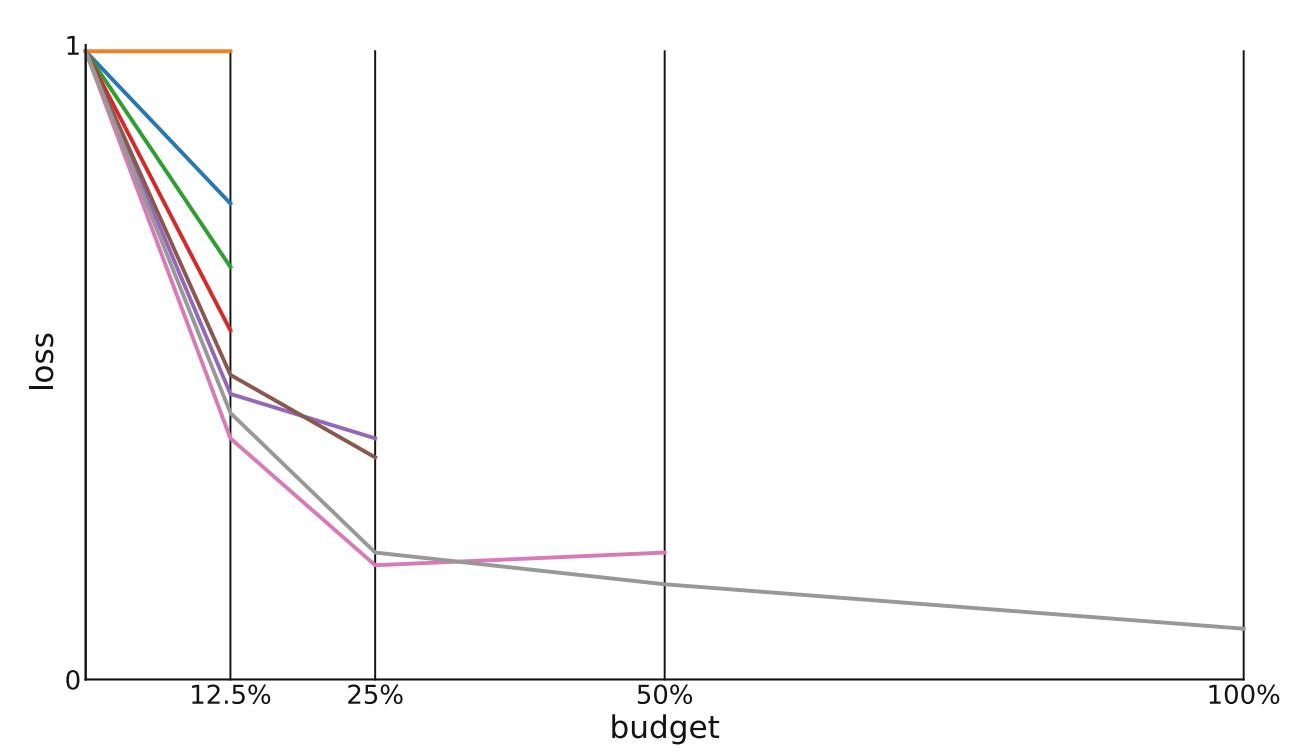
\includegraphics[width=\linewidth]{successive_halving}
    \caption{Illustration of successive halving for eight configurations. On each iteration, half of the algorithms are dropped while the resource budget for the remaining algorithms is doubled~\cite{Feurer.2019}.}
    \label{fig:succ_halving}
\end{figure}

\cite{Feurer.2019} gives a broad overview of the different kinds of hyperparameter optimization techniques. In this work, the HyperBand \cite{li2017hyperband} is used to optimize the hyperparameters. The algorithm is based on a successive halving approach, as shown in \autoref{fig:succ_halving}.
The training starts with $n$ different configurations, using $b=\frac{1}{n}$ of the available resources. After this training step, the configuration pool is halved, keeping only the best $n' = n/2$ configurations. At the same time, the resource budget for the remaining configurations is effectively doubled $b=\frac{1}{n'}=\frac{1}{\frac{n}{2}} = 2\times\frac{1}{n}$.
This process is repeated until a single best algorithm is left. Hyperband improves on this basic successive halving strategy by not only randomly sampling the available configurations in the parameter space but also the budgets assigned to the selected configurations. In practice, HyperBand has shown to increase performance with only a relatively small increase in computation time~\cite[p. 17]{Feurer.2019}.

\begin{table}[htb]
\centering
    \caption{Hyperparameter search space for Keras model tuning}
    \begin{tabular}{cl}
            \toprule
            parameter name       & search space                   \\ 
            \midrule
            \# deep layers       & {[}1, 2, 3, 4{]}               \\
            deep layer size      & {[}128, 256, 512{]}            \\
            \# cross layers      & {[}1, 2, 3, 4{]}               \\
            learning rate        & {[}0.0001, 0.001, 0.01, 0.1{]} \\
            optimizer            & adam, adagrad                  \\
            projection dimension & {[}32, 64, 128{]}              \\ 
            \bottomrule
        \end{tabular}
    \label{tab:hparam_space}
\end{table}


The implemented Deep \& Cross Network architecture was tuned using the parameter search space as shown in \autoref{tab:hparam_space}.  This large search space was explored using the mentioned HyperBand algorithm.
In \autoref{fig:rmse_it} one can see the results of the successive halving approach used in the HyperBand algorithm. The figure shows the Root Mean Squared Error (RMSE), which is the evaluation metric for regression problems, in relation to the number of training steps carried out on different model configurations. The evaluations were carried out at the end of each epoch, where the number of models at the subsequent epochs was reduced according to the algorithm. The figure shows all Hyperband runs conducted with slightly different setups, through each whole parameter search space, to show the sheer number of trainings and evaluations.

\begin{figure}[ht]
    \centering
    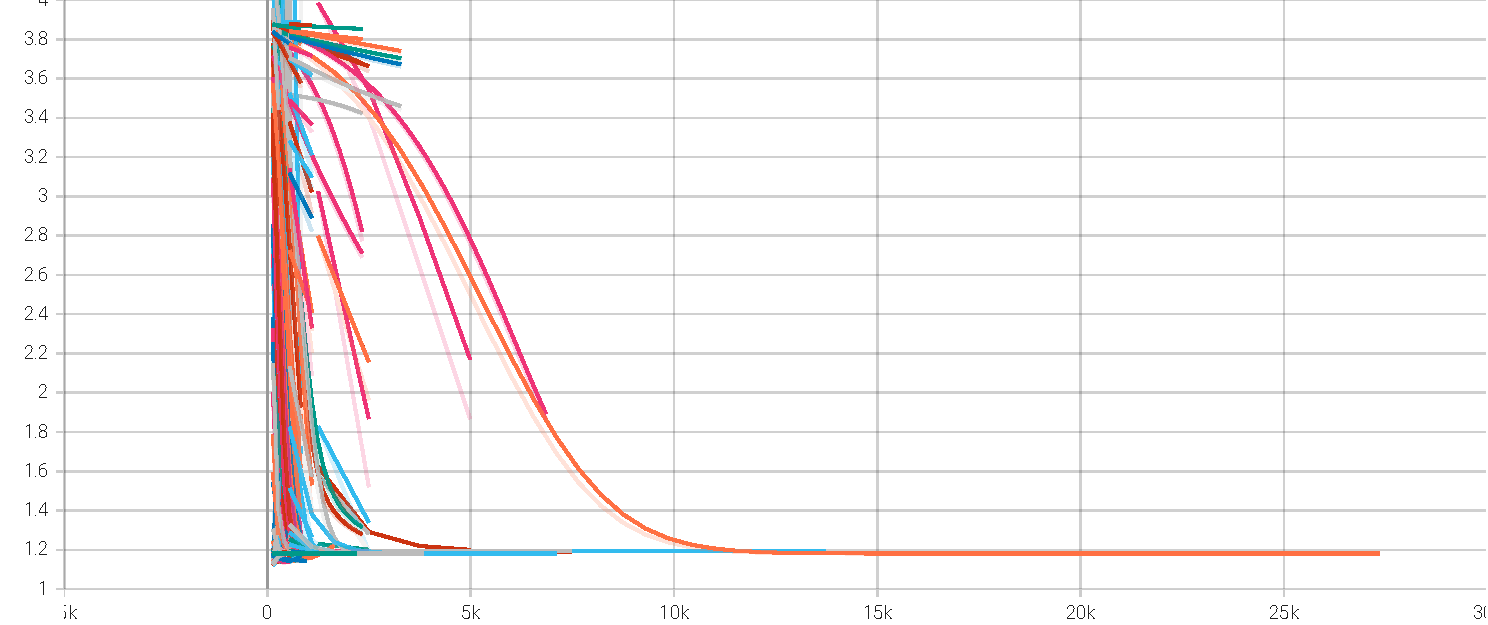
\includegraphics[width=\linewidth]{hp_tuning_20220_evaluation_root_mean_squared_error_vs_iterations.pdf}
    \caption{Evaluation results after number of training iterations. x-axis shows the number of steps, y-axis the evaluation metric Root Mean Squared Error (RMSE).}
    \label{fig:rmse_it}
\end{figure}

The parameter configurations of the top 50 best performing models can be found in \autoref{tab:hyp_table}. As one can see in the accompanying \autoref{fig:scatter}, there is no strong correlation between one specific parameter setting and better performance, since all variables are highly interdependent. That is why one can not define one general rule as to which parameter setting would be better because only certain specific combinations for this specific model and dataset work better.

\begin{figure}[ht]
    \centering
    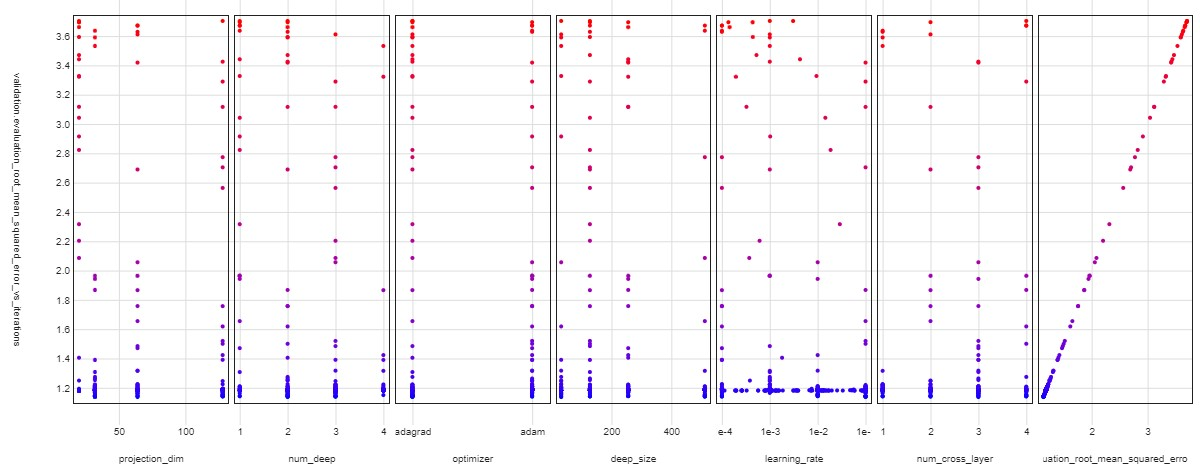
\includegraphics[width=\linewidth]{hparam_scatter.jpg}
    \caption{Scatter plot matrix showing the relationship between selected parameters and resulting RMSE}
    \label{fig:scatter}
\end{figure}


As can be seen in \autoref{tab:hyp_table} and in \autoref{fig:rmse_it}, of all the training efforts with different hyperparameter settings performed, the best settings always lead to the same resulting RMSE of about 1.14.
One advantage of RMSE is, that the resulting value is of the same unit as the input data, which means that the learned book ratings predicted for the test data presented to the neural network lie 1.14 points - or "stars" in the Goodreads nomenclature - off the actual ratings.
Working on a scale from 0 to 5, these results may be a bit disheartening, especially since none of the changes made to the network architecture seemed to have any positive effect breaking through this performance "barrier". Indeed, there were a few more experiments carried out, which will not be discussed here any further, using e.g. only a deep network architecture (with 0 number of cross layers), using an adaptive learning rate, using mean absolute error (MAE) instead of RMSE, and with only using ID data without complex text information. But unfortunately, none of those experiments lead to any better results, either.


\section{conclustion}
In this paper, the application of a neural network architecture developed in artificial intelligence and recommender systems research has been applied to a publicly available real-world dataset.
The major tasks in the field of data science, namely data preprocessing, data cleaning and model selection in the preparation stage, and finally model training and hyperparameter optimization have been carried out in this project and documented here.
Unfortunately, the results achieved by the trained neural network models still leave room for improvement. It goes to show, that the task of recommending a handful from thousands or millions of possible items is a very intricate problem to be solved, with no "go-to-solutions" available such as those that i.e. exist in the field of computer vision like image classification or object detection. 
Nevertheless, this paper documents the work already completed, and the code produced may be used to further improve the system, by either comparing it to other network architectures, using different word embeddings, or developing more problem-specific feature engineering approaches.

\bibliography{bibliography}
\pagebreak
\section*{appendix}
\begin{table}[hb]
    \centering
    \caption{Hyperparameter tuning top 50 results, sorted by evaluation RMSE}
    \label{tab:hyp_table}    
    \begin{tabular}{lllllll}
    \toprule
    num\_cross\_layer & optimizer & num\_deep & projection\_dim & deep\_size & learning\_rate & evaluation\_root\_mean\_squared\_error\_vs\_iterations \\ \midrule
    $3$ & adagrad & $2$ & $64$ & $32$ & $0.1$ & $1.14$ \\
    $2$ & adam & $3$ & $32$ & $512$ & $0.0001$ & $1.14$ \\
    $1$ & adagrad & $2$ & $128$ & $128$ & $0.1$ & $1.14$ \\
    $3$ & adagrad & $3$ & $32$ & $32$ & $0.1$ & $1.14$ \\
    $4$ & adagrad & $2$ & $128$ & $128$ & $0.1$ & $1.14$ \\
    $4$ & adagrad & $1$ & $32$ & $512$ & $0.1$ & $1.14$ \\
    $1$ & adagrad & $3$ & $32$ & $256$ & $0.01$ & $1.14$ \\
    $1$ & adagrad & $2$ & $128$ & $128$ & $0.1$ & $1.14$ \\
    $2$ & adagrad & $3$ & $64$ & $256$ & $0.01$ & $1.14$ \\
    $4$ & adagrad & $2$ & $128$ & $512$ & $0.01$ & $1.14$ \\
    $2$ & adagrad & $3$ & $128$ & $256$ & $0.1$ & $1.14$ \\
    $2$ & adam & $3$ & $32$ & $512$ & $0.0001$ & $1.14$ \\
    $3$ & adam & $2$ & $64$ & $512$ & $0.0001$ & $1.14$ \\
    $4$ & adagrad & $1$ & $32$ & $512$ & $0.1$ & $1.15$ \\
    $3$ & adam & $2$ & $64$ & $512$ & $0.0001$ & $1.15$ \\
    $4$ & adagrad & $4$ & $128$ & $32$ & $0.01$ & $1.15$ \\
    $2$ & adagrad & $2$ & $32$ & $128$ & $0.01$ & $1.15$ \\
    $3$ & adagrad & $2$ & $128$ & $256$ & $0.01$ & $1.15$ \\
    $4$ & adagrad & $2$ & $32$ & $32$ & $0.01$ & $1.15$ \\
    $4$ & adagrad & $3$ & $128$ & $512$ & $0.01$ & $1.15$ \\
    $3$ & adagrad & $3$ & $128$ & $512$ & $0.01$ & $1.16$ \\
    $3$ & adagrad & $2$ & $64$ & $32$ & $0.1$ & $1.16$ \\
    $1$ & adam & $3$ & $64$ & $128$ & $0.0001$ & $1.16$ \\
    $3$ & adam & $1$ & $64$ & $32$ & $0.01$ & $1.16$ \\
    $3$ & adam & $2$ & $32$ & $128$ & $0.001$ & $1.17$ \\
    $2$ & adagrad & $3$ & $128$ & $256$ & $0.1$ & $1.17$ \\
    $2$ & adagrad & $2$ & $128$ & $512$ & $0.001$ & $1.17$ \\
    $3$ & adam & $3$ & $32$ & $256$ & $0.0001$ & $1.17$ \\
    $3$ & adagrad & $3$ & $32$ & $32$ & $0.1$ & $1.17$ \\
    $4$ & adagrad & $2$ & $128$ & $128$ & $0.1$ & $1.17$ \\
    $1$ & adam & $3$ & $32$ & $256$ & $0.0001$ & $1.17$ \\
    $4$ & adam & $3$ & $64$ & $256$ & $0.0001$ & $1.17$ \\
    $3$ & adam & $3$ & $32$ & $32$ & $0.01$ & $1.18$ \\
    $3$ & adam & $2$ & $32$ & $512$ & $0.01$ & $1.18$ \\
    $2$ & adagrad & $2$ & $32$ & $32$ & $0.1$ & $1.18$ \\
    $2$ & adagrad & $2$ & $32$ & $32$ & $0.1$ & $1.18$ \\
    $1$ & adam & $3$ & $32$ & $512$ & $0.0001$ & $1.18$ \\
    $4$ & adam & $1$ & $32$ & $512$ & $0.1$ & $1.18$ \\
    $4$ & adagrad & $2$ & $64$ & $32$ & $0.1$ & $1.18$ \\
    $2$ & adagrad & $2$ & $32$ & $32$ & $0.1$ & $1.18$ \\
    $3$ & adam & $4$ & $32$ & $256$ & $0.01$ & $1.18$ \\
    $2$ & adagrad & $2$ & $32$ & $32$ & $0.1$ & $1.18$ \\
    $2$ & adam & $4$ & $32$ & $512$ & $0.01$ & $1.18$ \\
    $3$ & adagrad & $3$ & $32$ & $128$ & $0.1$ & $1.18$ \\
    $2$ & adam & $1$ & $32$ & $128$ & $0.1$ & $1.18$ \\
    $4$ & adagrad & $2$ & $64$ & $32$ & $0.1$ & $1.18$ \\
    $3$ & adam & $3$ & $32$ & $32$ & $0.01$ & $1.18$ \\
    $1$ & adagrad & $3$ & $64$ & $512$ & $0.001$ & $1.18$ \\
    $2$ & adagrad & $3$ & $128$ & $32$ & $0.01$ & $1.18$ \\
    $2$ & adagrad & $3$ & $128$ & $32$ & $0.01$ & $1.18$ \\
    \bottomrule
    \end{tabular}
\end{table}
\begin{table}
    \centering
    \caption{sample from the book data set}
    \label{tab:book_sample}
    \begin{tabular}{ll}
        \toprule
        name &                                                  value \\
        \midrule
        isbn                 &                                                    \\
        text\_reviews\_count   &                                                  7 \\
        series               &                                           [189911] \\
        country\_code         &                                                 US \\
        language\_code        &                                                eng \\
        popular\_shelves      &  [\{'count': '58', 'name': 'to-read'\}, \{'count':... \\
        asin                 &                                         B00071IKUY \\
        is\_ebook             &                                              false \\
        average\_rating       &                                               4.03 \\
        kindle\_asin          &                                                    \\
        similar\_books        &  [19997, 828466, 1569323, 425389, 1176674, 2627... \\
        description          &  Omnibus book club edition containing the Ladie... \\
        format               &                                          Hardcover \\
        link                 &  https://www.goodreads.com/book/show/7327624-th... \\
        authors              &               [\{'author\_id': '10333', 'role': ''\}] \\
        publisher            &                             Nelson Doubleday, Inc. \\
        num\_pages            &                                                600 \\
        publication\_day      &                                                    \\
        isbn13               &                                                    \\
        publication\_month    &                                                    \\
        edition\_information  &                                  Book Club Edition \\
        publication\_year     &                                               1987 \\
        url                  &  https://www.goodreads.com/book/show/7327624-th... \\
        image\_url            &  https://images.gr-assets.com/books/1304100136m... \\
        book\_id              &                                            7327624 \\
        ratings\_count        &                                                140 \\
        work\_id              &                                            8948723 \\
        title                &  The Unschooled Wizard (Sun Wolf and Starhawk, ... \\
        title\_without\_series &  The Unschooled Wizard (Sun Wolf and Starhawk, ... \\
        \bottomrule
        \end{tabular}
        
\end{table}

\begin{table}
    \label{tab:review_sample}
    \caption{sample from the review data set}
    \begin{tabular}{ll}
        \toprule
        name &                                                  value \\
        \midrule
        user\_id      &                   8842281e1d1347389f2ab93d60773d4d \\
        book\_id      &                                            4986701 \\
        review\_id    &                   bb7de32f9fadc36627e61aaef7a93142 \\
        rating       &                                                  4 \\
        review\_text  &  Found the Goodreads down image in this, and ma... \\
        date\_added   &                     Thu Aug 04 10:02:02 -0700 2011 \\
        date\_updated &                     Thu Aug 04 10:02:02 -0700 2011 \\
        read\_at      &                                                NaT \\
        started\_at   &                                                NaT \\
        n\_votes      &                                                  6 \\
        n\_comments   &                                                  4 \\
        \bottomrule
        \end{tabular}
        
\end{table}
\end{document}
